% Lesson 4

\chapter{Cuarta Lección} % Chapter title

\label{ch:lesson04} % For referencing the chapter elsewhere, use \autoref{ch:examples} 

%----------------------------------------------------------------------------------------

% =====================
% 		GRAMATICA
% =====================
\Large{\section*{Gramática}}

\bemph{\subsection*{Caso Nominativo Singular}}

\S\ 20. La forma del caso nominativo de ambos sustantivos y adjetivos no tiene una terminación en particular. Puede terminar en casi cualquier vocal o consonante.\\

\begin{center}
\begin{tabular}{ l }
	 \bemph{isa} `padre', \bemph{õde} `hermana', \bemph{käsi} `mano', \bemph{töö} `trabajo', \\ 
	 \bemph{vana} `viejo/vieja', \bemph{terve} `saludable', \bemph{hea} `bien', \bemph{mees} `hombre', \\
	 \bemph{sõber} `amigo', \bemph{raamat} `libro', \bemph{noor} `joven', \bemph{paks} `gordo/gorda', \\
	 \bemph{kõhn} `delgado/delgada', \bemph{vend} `hermano', \bemph{laps} `niño/niña'
\end{tabular}
\end{center}
\bigskip

\S\ 21. El caso nominativo (\bemph{nimetav kääne} en estonio) responde a las preguntas \bemph{kes?} `¿quién?', \bemph{mis?} `¿qué?', \bemph{milline?} (o \bemph{missugune?}) `¿qué tipo?'. Se utiliza principalmente para los sujetos de las oraciones y los complementos del predicado.\\

\begin{center}
\begin{tabular}{ l l }
	\bemph{Kes} kirjutab?	&	`¿Quién escribe?' \\
	\bemph{Vend} kirjutab.	&	`El hermano escribe.' \\
	&  \\		
	\bemph{Kes} ta on?		&	`¿Quién es él/ella?' \\
	Ta on \bemph{õpetaja}.	&	`Él/Ella es un/una profesor/profesora.' \\
	&  \\	
	\bemph{Milline} ta on?	&	`¿Qué tipo es él/ella?' (¿Cómo es él/ella?)' \\
	Ta on \bemph{noor}.		&	`Él/Ella es joven.' \\
	&  \\
	\bemph{Mis} seal on?	&	`¿Qué es eso?' \\
	Seal on \bemph{laud}.	&	`Eso es una mesa.' \\
	&  \\
	\bemph{Mis} see on?		&	`¿Qué es eso?' \\
	See on \bemph{raamat}.	&	`Eso es un libro.' 
\end{tabular}
\end{center}
\bigskip

\S\ 22. Al igual que en español, el verbo se conjuga de acuerdo al pronombre personal y no a la palabra `Ese' en las cláusulas del tipo `Ese soy yo'. \\

\begin{center}
See \bemph{olen mina}. `Ese soy yo.' See \bemph{oled sina}. `Ese eres tú.' See \bemph{on tema}. `Ese es él/ella.'
\end{center}

\S\ 23. En una oración negativa, se usa a menudo una doble negación. El español no tiene tal partícula, pero equivaldría a recalcar la partícula negativa de la oración. Esto quiere decir que en el estonio la doble negación sigue siendo negativa, utilizando la partícula \bemph{mitte} para reforzar el impacto negativo del \bemph{ei}.\\

\begin{center}
\begin{tabular}{ l l }
	Ma \bemph{ei} tea \bemph{mitte midagi}.			& `Yo no sé \bemph{nada}.' \\
	&  \\
	Ta \bemph{ei} tule \bemph{mitte iialgi} tagasi. & `Él/Ella \bemph{nunca} volverá.'
\end{tabular}
\end{center}
\bigskip

% ==================
% 		TEXTO
% ==================
\Large{\section*{Texto}}

Vend on juba suur poiss. Ta käib koolis. Õde on väike tüdruk. Ta mängib kodus. Ta on hea laps. Vanaisa ja vanaema istuvad ja puhkavad. Nad vaatavad pealt kuidas väike laps mängib. Tädi ja onu tulevad homme külla. Siis on ka vanemad kodus.\\
Kas isa on vana mees? Ei ole, isa on veel noor inimene. Ema on ka noor. Ema on noor naine. Onu on aga juba vana mees. Milline on tädi? Tädi on noor ja ilus. \\

\begin{center}
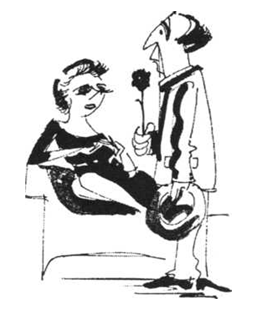
\includegraphics{img/L04.png}
\end{center}
\bigskip

\noindent
-- Mida te teete, proua Kivisaar, et te nii noor ja ilus välja näete? \\
-- Ma ei tee mitte midagi. \\

\noindent
Rumal räägib, mis ta teab, tark teab, mis ta räägib. \\
Kõik pole kuld, mis hiilgab, (Vanasõna) \\
Üles läheb, alla ei tule. (Mõistatus) -- Suits. \\

% =======================
% 		VOCABULARIO
% =======================
\Large{\section*{Vocabulario}}

\begin{tabular}{ l l }
alla			&	abajo \\
hea				&	bien, bueno \\
hiilga/n		&	(Yo) brillo \\
ilus			&	hermosa, linda \\
inimene			&	persona \\
juba			&	ya (\eg ya estoy listo) \\
koolis			&	en el colegio  \\
kuld			&	oro \\
kõik			&	todo \\
käi/n koolis	&	(Yo) voy al colegio \\
külla			&	de visita \\
laps			&	niño/niña \\
mees			&	hombre \\
mida [= mis]	&	qué \\
midagi			&	algo, nada \\
milline			&	qué tipo \\
mitte			&	(reforzador de negación) \\
mitte midagi	&	(absolutamente) nada \\
mõistatus		&	acertijo  \\
mängi/n			&	(Yo) juego \\
naine			&	mujer \\
noor			&	joven \\
näe/n välia		&	(Yo) parezco, Me veo \\
onu				&	tío \\
proua			&	Sra. (Señora) \\
rumal			&	(persona) estúpida  \\
suits			&	humo \\
suur			&	grande \\
tark			&	(persona) astuta, inteligente  \\
tädi			&	tía \\
vaata/n pealt	&	(Yo) observo \\
vana			&	viejo/vieja \\
vanaema			&	abuela \\
vanaisa			&	abuelo \\
vanasõna		&	proverbio, dicho antiguo \\
vanemad			&	padres, ancianos \\
väike			&	pequeño \\
üles			&	arriba
\end{tabular}
\bigskip

% ======================
% 		EJERCICIOS
% ======================
\Large{\section*{Ejercicios}}

\begin{enumerate}
	\item \emph{Traducir al estonio:} ¿Qué es esto? Este es una tabla. ¿Quién está allí? Soy Yo. ¿Quién va a la escuela? Él es un buen chico. ¿La pequeña hermana también va a la escuela? No, ella no va a la escuela todavía. Ella es una niña. Hermano y hermana juegan en casa. ¿Van ustedes a casa? Vamos a estar en casa mañana. El abuelo es un hombre viejo. La sra. Kivisaar es una mujer joven. Ella es muy bonita. ¿El tío es joven? No, no es joven, ya es viejo. ¿Es muy viejo? No, no lo es. ¿Qué está haciendo la tía hoy? No sé. ¿Entiendes lo que digo? ¡Di algo! ¡No hables en voz tan baja!

	\item \emph{Traducir al español:} 

	\begin{center}
	\begin{tabular}{ l l }
		mees -- naine		& poeg -- tütar \\  
		poiss -- tüdruk   	& vend — õde \\ 
		isa -- ema 			& onu -- tädi \\
		vanaisa — vanaema	& laps -- vanemad - perekond
	\end{tabular}
	\end{center}
	\bigskip
\end{enumerate}

% ============================
% 		EXPRESIONES DE ...
% ============================
\Large{\section*{Expresiones de Curiosidad}}

\begin{tabular}{ l l }
	Mis see on?							& ¿Qué es esto? \\
	Mis see tähendab?					& ¿Qué significa esto? \\
	Kes seal on? Kes see on? 			& ¿Quién está allí? ¿Quién es (este)? \\
	See on härra/proua/preili... 		& (Este) es el/la señor/señora/señorita ...\\
	Kas see on proua Palm?				& ¿Es (esta) la señora Palm? \\
	Jah, on küll. -- E¡ ole.			& Sí, lo es. -- No lo es. \\
	Kuidas te teate?					& ¿Cómo saben? \\
	Mis sa arvad? Mis te arvate?		& ¿Qué crees tú? ¿Qué creen ustedes? \\
	Kas sa saad aru? Kas te saate aru? 	& ¿Entiendes? ¿Entienden? \\
	Saan aru. -- Ma ei saa aru.			& Entiendo -- No entiendo \\
	Kuidas, palun?						& ¿Disculpa? (¿qué dijiste?) \\
	Vabandust, ma ei kuulnud.			& Perdón, no escuché. \\
	Palun korda! Palun korrake!			& ¡Por favor repite! ¡Por favor repita!  
\end{tabular}
\bigskip

% ======================================
% 		RESPUESTA A LOS EJERCICIOS
% ======================================
\Large{\section*{Respuesta a los ejercicios}}

\begin{enumerate}
	\item Mis see on? See on (üks) laud. Kes seisab seal? See olen mina. Kes käib koolis? Ta on hea poiss. Kas väike õde käib ka koolis? Ei, tema ei käi veel koolis. Ta on väike tüdruk. Vend ja õde mängivad kodus. Kas te lähete koju? Me oleme homme kodus. Vanaisa on vana mees. Proua Kivisaar on noor naine. Ta on väga ilus. Kas onu on noor inimene? Ei, ta pole [= ei ole] noor, ta on vana. Kas ta on väga vana? Ei ole. Mis tädi teeb täna? Ma ei tea. Kas sa saad aru, mis ma ütlen? Ütle midagi! Ära räägi nii tasa!

	\item 
	\begin{tabular}{ l l }
		hombre -- mujer		& hijo -- hija \\
		niño -- niña		& hermano -- hermana \\
		padre -- madre		& tío -- tía \\
		abuelo -- abuela	& laps -- vanemad -- perekond 
	\end{tabular}
\end{enumerate}

%----------------------------------------------------------------------------------------